
\documentclass[conference]{acmsiggraph}

\usepackage{enumitem}

\TOGonlineid{45678}
\TOGvolume{0}
\TOGnumber{0}
\TOGarticleDOI{1111111.2222222}
\TOGprojectURL{}
\TOGvideoURL{}
\TOGdataURL{}
\TOGcodeURL{}

\title{Real-time gait control for partially immersed bipeds}
% *** Walk Motion Control in Partial Immersion - à décider à la fin ***

\author{Samuel Carensac\thanks{e-mail:samuel.carensac@gmail.com}, Nicolas Pronost, Saida Bouakaz\\University Claude Bernard Lyon 1, LIRIS}
\pdfauthor{Samuel Carensac}

\keywords{Virtual Human, Physics-based animation, Motion control, Real-time liquid interaction, Offline optimization}

\begin{document}

\teaser{
   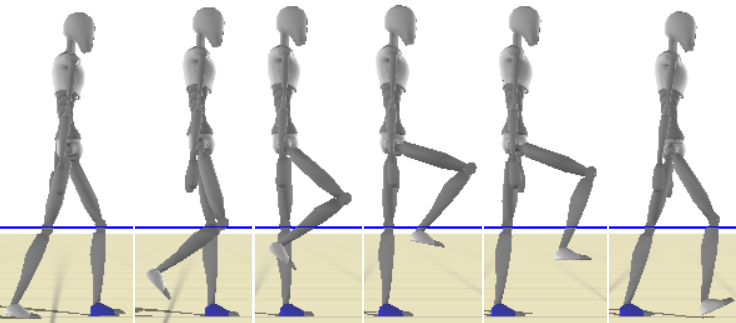
\includegraphics[height=1.5in]{images/3_6_1_50cm.png}
   \caption{Real-time physics-based simulation of walking of a partially immersed biped. Our method provides robust balance, adaptive gait style to environment and precise speed tracking. ***Not final image (need longer series)***}
	% *** Peut-être trouver une série où le pied sort complètement de l'eau ***
\label{fig:intro}
}

\maketitle

\begin{abstract}

Physics-based animation is an increasingly studied subject because it allows natural interactions with the virtual environment. Though some existing motion controllers can handle the simulation of interactions between a character and a liquid, only few methods focus on the simulation of the locomotion of immersed bipeds. In this paper, we present a control strategy capable of simulating partially immersed gaits. The impact of the liquid on the character's motion is modeled through simple hydrodynamics. We designed a controller allowing the combination of multiples gait styles, the conservation of balance through intelligent foot placement and precise control of the character's speed. We determined the optimal parameters for the controller by using an optimization process. This optimization has been repeated for several scenarios where the character has to walk across a volume of liquid parametrized by its height. Finally our controller is capable of online adaptation to the variation of liquid height, to the modification of the liquid density and to the variation of the required character speed.

\end{abstract}

\begin{CRcatlist}
  \CRcat{I.3.3}{Computer Graphics}{Three-Dimensional Graphics and Realism}{Animation}
\end{CRcatlist}

\keywordlist

\copyrightspace

\section{Introduction}

Simulating realistic human motion is a key step in creating virtual environments. Over the years, these environments have become increasingly diverse and complex with large numbers of elements that can influence the motion of a virtual character. In those cases, physics-based animation are preferred over kinematic animation since it doesn't need a series of exact position for each possible interaction. With this increasing complexity, it is now difficult to achieve realistic interactions between animated characters and the environment using kinematics-based approaches. Physics-based animation uses physical phenomena (forces and torques) to manipulate the character. This allows the creation of a motion that will be directly impacted by the environment. A growing number of contributions are now working on building physics-based controllers~\cite{geijtenbeek2012interactive}. Although they inherently allow obtaining interactions with the environment, the manipulation of the character becomes more complex as no direct control over the position of the limbs of the animated characters is possible.

The main challenge of a controller is to allow high level parametrization of the system under the constraint of partial immersion. For example, these high level parameters may be the character's speed, the direction of displacement or the motion style. The need to simulate a large number of motion styles (walking, running, jumping...) makes creating a generic controller extremely challenging. Similarly, the mastery of multiples interactions with the environment also increases considerably the complexity of the system. This is why the existing controllers focus on the study of a limited number of motion styles at a time and interactions with the environment~\cite{geijtenbeek2012interactive}. We focused on the control of walking in partial immersion conditions in a liquid. Our objective was to define and implement the necessary mechanisms to a physics-based controller to allow real-time animation of a virtual character interacting with a liquid. Our controller is capable of great freedom of gait style and precise tracking of the character's motion speed.

This paper will start by presenting the existing works related to our contributions (section~\ref{sec:previous_works}). Section~\ref{sec:overview} proposes a global view of our system followed by a detailed description of each component in sections~\ref{sec:ext_forces} and~\ref{sec:control_framework}. We present our results and the limits of our method in section~\ref{sec:results} then finish by a short conclusion (section~\ref{sec:conclusion}).
 
\section{Previous works}
\label{sec:previous_works}

Numerous works on control of virtual characters with simulated physics can be found in the literature~\cite{geijtenbeek2012interactive}. Among those works, some share common characteristics with our objectives.

Our work share some features of the SIMBICON (SIMple BIped CONtroler)~\cite{yin2007simbicon} and associated works. Among them, \cite{coros2009robust} propose a system integrating multiples controllers for navigation task. The drawback is that the system is designed to use optimization to determine how the different controllers should be used. To enable the use of low gains in the PD-controllers different methods have been used such as a feedforward system~\cite{yin2007simbicon} or the computation of torques to compensate the effect of gravity~\cite{coros2010generalized}.

\textbf{\textit{Balance control}} is one of the key systems in physics-based simulation. The original SIMBICON uses for instance secondary PD-controllers on the key joints (stance ankle and swing hip) to dynamically adapt the tracked positions. One way to compute a balance aware foot placement during walk motion is to use an Inverted Pendulum Model (IPM)~\cite{coros2010generalized,kajita20013d}. The IPM can be used to dynamically compute the trajectory of the swing foot but it limits the range of possible gaits styles.

\textbf{\textit{Velocity control}} is often one of the required characteristics of physics-based controllers. Some works propose systems capable of adapting to online variations of the desired velocity. \cite{coros2009robust} obtains it by combining multiple controllers for specific motions (e.g. walk forward and walk backward). The IPM based systems offers an inherent, though imprecise as it does not consider the observed velocity, control~\cite{coros2010generalized}. The use of horizontal virtual forces has been a way to obtain a precise control of the speed and balance of the character~\cite{coros2010generalized,geijtenbeek2012simple}. This system is based on secondary PD-controllers to compute the necessary force. The static gains and constant used in those systems make them unable to track correctly the desired speed when the character is subject to a variable environment (e.g. apparition of a liquid medium). 

\textbf{\textit{Movement in liquids}} have been studied in both simulation~\cite{yang2004layered,si2014realistic} and biomechanics~\cite{barela2006biomechanical,chevutschi2009comparison}. Those works mainly focus on swimming control for simulation works and walk study with high level of immersion for biomechanics studies making them unusable in our scenarios. Other approaches worked on simulating human walk under wind forces~\cite{lentine2011creature}. Most of those works use the Navier-Stockes equations to simulate the liquids making them unfit to obtain real-time and interactive simulations.

In this paper we propose a new controller showing the following characteristics:
\begin{itemize}
\item{real-time interactive simulation by using simple hydrodynamics to simulate the impact of the liquid}
\item{dynamic gait style adaptation by combining multiple reference controllers}
\item{liquid impact aware gait styles by specific IPM usage and offline optimization}
\item{precise tracking of desired velocity by using learning strategies}
\end{itemize}

\section{Overview}
\label{sec:overview}

\begin{figure}[t]
\centering
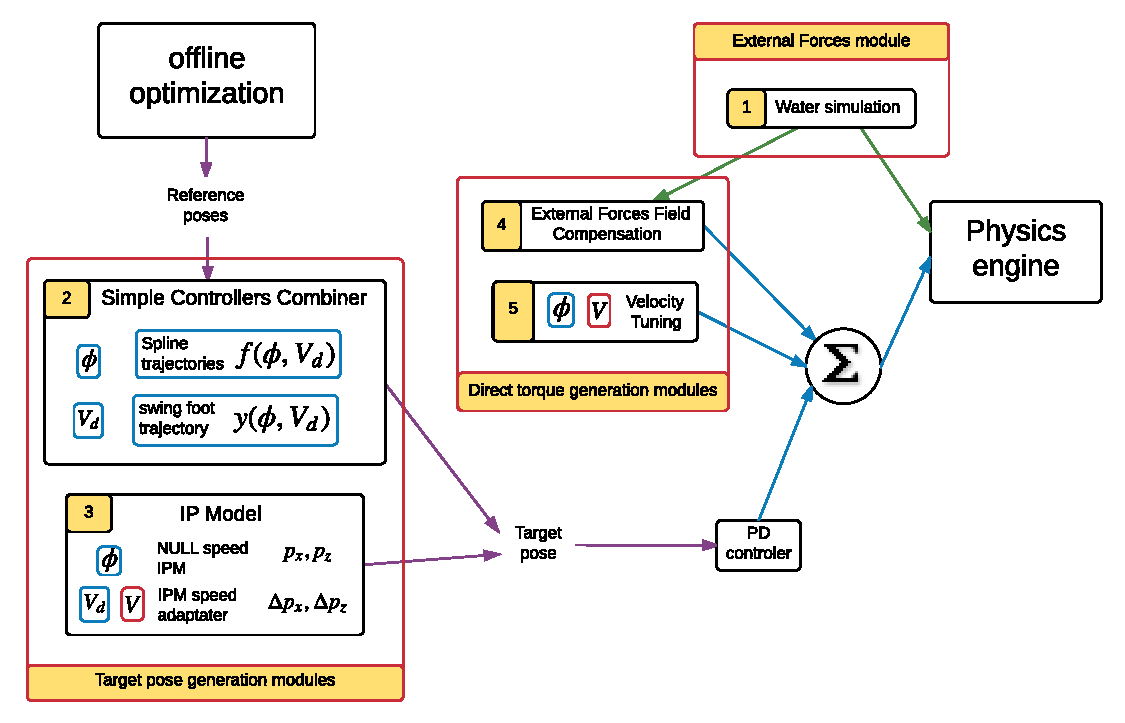
\includegraphics[scale=0.45]{images/general_process.pdf}
\caption{System Overview. The key components of the system are: (1) influence of liquid through external forces; (2) a combination of controllers generating the target poses; (3) an IPM for predictive foot placement; (4) an external force-field compensation helping the PD-controller; (5) velocity tuning for fine velocity and balance corrections.}
\label{fig:shema_controler}
\end{figure}

Our controller consists of five key components that are classified in three categories (figure \ref{fig:shema_controler}).

We start by simulating the liquid impact on the character by applying external forces computed by simple hydrodynamics (drag, friction and buoyancy) allowing us to obtain real-time interactions between the liquid and the character (section~\ref{sec:ext_forces}).
We use a combination of various controllers each one defining a gait style depending on simulation conditions (e.g. liquid level, desired speed) allowing an adaptive evolution of the gait style (section~\ref{sec:multi_state}). The specified trajectories for the joints composing the swing leg are overridden by the results of an IPM if the character is in the falling phase of a step or if the controller detects a loss of balance (section~\ref{sec:specific_ipm}).

We augment the PD-controller with torques computed through an external force-field compensation. This system is a generalization of Coros et al.'s gravity compensation mechanism~\cite{coros2010generalized} and helps us compute a significant part of the necessary torques (section~\ref{sec:ext_force_comp}).

Our controller includes a precise tracking of the desired velocity through an adaptive offset on the swing foot position computed by the IPM (section~\ref{sec:ipm_alt}). We also propose an amelioration of Coros et al.'s fine-scale control~\cite{coros2010generalized} by considering the intra-step speed variation of the character to compute a more efficient virtual force (section~\ref{sec:speed_virt_force}).

Finally, we use offline optimization to generate the reference poses used by the controller combinator. This optimization defines a gait style specific to a desired scenario (section~\ref{sec:optimisation}).

\section{External Forces}
\label{sec:ext_forces}

Beside the ground reaction forces, the external forces generated in our simulations are the forces related to the influence of the liquid on the character. To compute these forces, we use hydrodynamics laws by considering two types of forces. The first one is buoyancy. We use the well-known equation $F_{B}=-V_i \rho g$ with $V_i$ the immersed volume of the physics representation of the immersed object. The second type of forces is the parasitic drag. We restrict the considered physics phenomena to the form drag and the skin friction, modeling the resulting force $F_D$ using the following equation:
$$
F_D=\frac{1}{2} \rho v^2 A_n C_d \times \mu
$$
Where $C_d$ is the drag coefficient, $\rho$ the fluid density, $A_n$ the cross sectional area and $v$ the relative speed to the fluid. Due to the complexity of dynamically computing $C_d$, we set it to 1.0 (average value for a man). $\mu$ is a simple coefficient representing the fluid viscosity allowing us a rough representation of the friction. The velocity varying through the limbs we use a finite elements decomposition of the surface of each limb and compute the parasitic drag for each element. As such the computation of the cross sectional area $A_n$ and the immersion test are directly realized on each element.

\section{Control Framework}
\label{sec:control_framework}

Our system is built on the version of SIMBICON presented in~\cite{coros2010generalized}. The trajectories for the ankles, pelvis, back and head are specified in the coordinate system of the character. This coordinate system is similar to the global one but the z-axis indicates the direction that the character is currently facing. The trajectories for the shoulders, elbows, toes and the knee of the stance leg are specified using each joint local coordinates. Unlike~\cite{coros2010generalized}, we allow manual specification of the swing foot trajectory. This specification is made in the local coordinate system of the swing hip.

\subsection{Simple Controllers Combiner}
\label{sec:multi_state}

The \textit{Simple Controllers Combiner} allows us to observe dynamic variations of the gait style depending on the conditions of the simulation (e.g. liquid level). The principle is to use multiple simple controllers that are specified for one set of conditions. For this work, we limit the conditions to the walking speed and the liquid level but the system could handle other specifications. Each simple controller defines the trajectories for the joints that exhibit significant variations from one standard controller. For example, our standard controller is a forward walking controller and as such it specifies that the heel hits the ground before the toes do. If we want to be able to walk backward we will have to specify a simple controller specifying that the toes hit the ground before the heel and affect it a negative sagittal speed. Our system differs from the one presented in~\cite{coros2009robust} by two characteristics. First, we do not require each individual controller to produce a stable motion. In our system the balance is acquired by the use of an IPM. Second, each individual controller only specifies the joints where the variation from the standard state is significant. On a more conceptual view, in our system, we just want to specify the variations of the gait and not the variations of control strategy. Also we do not require an optimization step to find the optimal combination of the simple controllers. When the character ends a step, the system will compute a new trajectory for each joint. To find those trajectories we use an interpolation following a square-law between the trajectories specified for the two nearest simple controllers. For example, if we use controllers defined only by their reference speeds, we will use the two controllers $f_1$ and $f_2$ defined for the speeds $V_1$ and $V_2$ that are the nearest from the desired speed $V_d$ respecting $V_1 < V_d < V_2$. If we cannot find two speeds respecting this rule we directly use the nearest simple controller. The following equation gives how the resulting trajectories $f$ are computed:
$$
f=f_1*(1-R)+f_2*R   \quad \textrm{with} \quad   R=\left( \frac{V_d-V_1}{V_2-V_1} \right) ^2
$$

\subsection{Inversed Pendulum Model}
\label{sec:IPM}

We use an \textit{Inversed Pendulum Model} (IPM) supposing constant leg size and zero desired velocity similar to the one used in~\cite{coros2010generalized}. We have modified this model to allow the specification of previously impossible gaits styles and to enable a better tracking of the user's desired velocity. 

\subsubsection{Specific IPM Usage}
\label{sec:specific_ipm}

Our idea to enable the specification of new gait style is that the IPM does not need to control the swing foot during the whole step. We only need to control the position of the swing foot when the character is in a falling state, meaning when the vertical speed of the center of mass is positive $V_{COM}>0$. During a step, the falling phase corresponds to the end of the step. So during the first part of the step we will use a user defined trajectory for the swing foot. This allows the observation of vertical movement of the swing foot without any horizontal movement, which was previously impossible. This kind of gait style is important in our scenarios as it is typical of a character trying to minimize the drag from moving in a liquid (Figure~\ref{fig:intro}).

\subsubsection{IPM Result alteration}
\label{sec:ipm_alt}

To have a partil control of the velocity ~\cite{coros2010generalized} uses a linear modification of IPM results depending on the desired character velocity ($\Delta=-\alpha V_d$). The major flaw of their system used in is that it only functions properly near the velocity for which the linear factor used has been optimized. 

In particular, this system cannot handle the transition from an environment with a fluid medium to an unconstrained one. Our solution is to add a supplementary offset $\Delta(x,z)$ to the results of the IPM. This offset will be modified at the end of each step depending on the difference between the current character velocity and the desired velocity $\Delta(x,z) = \Delta(x,z)+\beta(V-V_d)$ with $\beta$ a positive constant. The swing foot position from the IP model $P_{IPM}(x,z)$ will therefore be modified as follows:
$$
P(x,z) = P_{IPM}(x,z) - \alpha V_d + \Delta(x,z)
$$ 

\subsection{External Force Fields Compensator}
\label{sec:ext_force_comp}

Our \textit{External Force Fields Compensator} is an extension of the gravity compensation proposed in~\cite{coros2010generalized}. The goal is to dynamically compute a part of the necessary torques at each joint thus permitting the use of lower gains in the main PD-controller. Using virtual forces oposing the diverse external force fields affecting the character gives us a decent and quick to compute series of torques fiting that desciption.
The external forces that we consider are the weight $P=mg$ of each body part of the character and buoyancy $F_B=-\rho V_i$. We chose to ignore the liquid drag in the compensator because it would imply the use of many small forces (depending on the precision of the finite elements)  which would be time consuming to compensate with our method.
So the final virtual force applied to each body part is:
$$
F=-mg+\rho V_i
$$

\subsection{Velocity Tuning}
\label{sec:speed_virt_force}

\begin{figure*}[t]
\centering
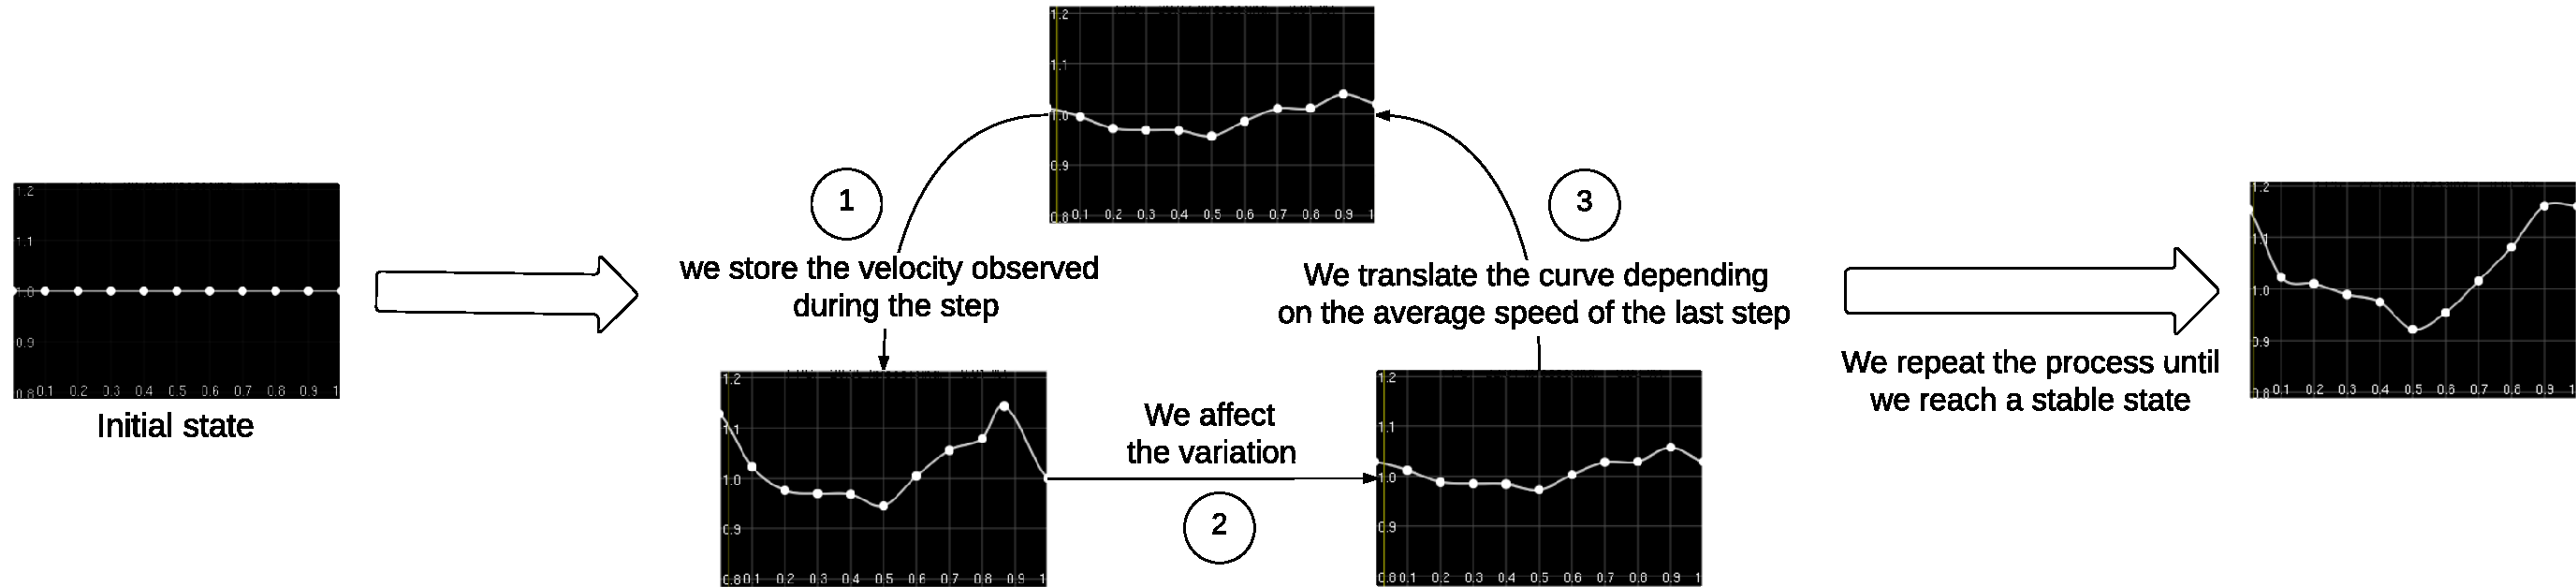
\includegraphics[scale=0.35]{images/speed_curve_learner.pdf}
\caption{Process of learning the adapted required velicity curve}
\label{fig:speed_curve_learner}
\end{figure*}

Similarly to the velocity tuning in~\cite{coros2010generalized}, ours applies a horizontal virtual force to obtain a fine control of the speed and balance. Our version presents three major differences. First, we do not consider the same chain of limbs. Instead of considering one chain that goes from the head to the stance foot we use two: one going from the pelvis to the stance foot and one made of the torso alone. This modification comes from two considerations. First, we do not consider the head in the top chain because we do not want the character to tilt the head to control its velocity. Second, we separate the torso from the lower body because we estimate that the main control strategy of the speed should be to simply tilt the torso and not to exert huge torques on the stance ankle. To do so, our Jacobian matrix takes into account the mass $M_i$ of each individual limb:
$$
J_n ^T (p)=\frac{1}{M}\sum_{\substack{0<i\leq n}} ((P_i(x,y,z)-P_{i-1}(x,y,z))*M_i)
$$
Where $M$ is the mass sum of the limbs considered in the velocity tuning, $P_i(x,y,z)$ the position of the $i$ joint and $P_0(x,y,z)$ the application point of the virtual force. This modification allows us to give more importance to the joints controlling a lot of mass (i.e. the joint between the pelvis and the torso).

We also consider the intra-step velocity variations. In most cases, the velocity is not constant during a step. Supposing it constant as ~\cite{coros2010generalized} may cause the apparition of undesired behavior where the controller asks the character to slow at the start of the step, then accelerate when near the middle of the step to slow once again near the foot strike. This is why we use a system to learn a curve specifying the needed velocity at each instant of a step to produce a virtual force as constant as possible. This learning velocity curve is defined by $k$ key points equaly dispersed. The values between those points are computed by using Catmull-Rom splines. Our tests have shown that a value of $k=11$ give enougth precision without being time consuming. The learning method is based on an iterative principle. During a step we record the velocity of the center of mass. When the step ends we check if the average variation between the learning velocity curve and the observed velocity is lower than a threshold. If it is we evolve the learning velocity curve so that it fits the observed one. Then we adapt the learning curve depending on the ratio between the desired velocity and the average observed velocity $R=V_d/V_{avg}$ (see figure \ref{fig:speed_curve_learner}). If the variation is higher than the threshold it means the character is not in a stable motion anymore. In that case we stop adapting our learning curve and switch to the use of recovery steps, meaning the full trajectory of the swing foot will be defined by the IPM. We stay in recovery mode until the average variation between the observed speed and the specified one is lower than the threshold. If it takes more than five steps we reset the learning curve to the constant desired value and we start learning again. Our system uses one learning curve for the sagittal speed and two curves of the coronal speed (one for each stance).
% *** Ce paragraphe n'est pas très clair *** mieux maintenant? ***

\subsection{Offline Optimisation}
\label{sec:optimisation}

The goal of our offline optimization is to find the various simple controllers that we will use as input.
The considered parameters during our optimization are the swing foot trajectory and the coronal component of the angular trajectory for the following joints of elements:
\begin{itemize}[noitemsep,nolistsep]
\item{pelvis (3 key points);}
\item{joint between the pelvis and the torso (2 key points);}
\item{stance ankle (11 key points );}
\item{swing ankle (11 key points);}
\item{stance knee (5 key points);}
\end{itemize}
The swing foot trajectory is defined by respectively 3, 5 and 11 key points for the x, y and z axis. So our optimization considers a total of 51 variables.


\subsubsection{Objective function}
During our optimization we use the following evaluation function:
\begin{equation}
\begin{split}
f_{eval} &=\sum_{\substack{t<k}} (\alpha f_{energ} + \beta f_{drag} + \gamma f_{acc})\, *\\&(1+0.1* R_{ipm\_alt}) 
+ f_{speed} + f_{balance}
\label{eq:complete_eval}
\end{split}
\end{equation}
With $k$ the duration in second of the evaluation. This function can be separated in two parts, each one composed of three functions. The first part corresponds to the sum and defines the characteristics that we want to appear once the optimization finished. To do so we use a weighted sum of three functions, each one defining a specific behavior:
\begin{itemize}
\item{\textit{Minimization of consumed energy} ($f_{energ}$). The goal of this function is to obtain a motion using the minimum energy possible. This function is evaluated by the sum of the torques at every joint $f_{energ}=\sum_{\substack{i}}{\tau_i}$} 
\item{\textit{Minimization of the drag}. ($f_{drag}$). This function result in a motion that tries to stay away from the liquid and prevents the velocity spikes inside the liquid. We evaluate it by using the sum of the torques induced by the drag forces on the parent joint of the limb where the drag forces are applied ; $f_{energ}=\sum_{\substack{i}}\sum_{\substack{j}}((P_j(x,y,z)-P_i(x,y,z)) \times F_j)$ with  $P_j(x,y,z)$ the force application point and $P_i(x,y,z)$ the position of the parent joint.}
\item{\textit{Minimization of angular acceleration} ($f_{acc}$). The goal of this function is to obtain a smooth motion.Thi function is evaluated by the sum of the angular acceleration on the reference poses $\ddot{\theta_d}_i$ and on the resulting motion $\ddot{\theta}_i$. To favor minimizing the acceleration of the actual motion we give them a factor of 0.75 and a factor of 0.25 to the reference poses; $f_{acc}=0.25*\sum_{\substack{i}}\ddot{\theta_d}_i+0.75*\sum_{\substack{i}}\ddot{\theta}_i$ }
\end{itemize}

The second part of the evaluation function consists in function limiting the research space:
\begin{itemize}
\item{\textit{Penalization of IPM alteration} ($R_{ipm\_alt}$). The IPM alteration system is powerful, way too powerful in fact. Even with references poses defined to walk backward our system could succeed in walking forward if asked. To prevent this kind of situations, we penalize simulation if it relies heavily on the IPM alteration. To evaluate this function we use the ratio between the needed IPM alteration $\Delta(x,z)$ to obtain a stable motion and the maximum possible value $max(\Delta(x,z))$ (0.09);  $R_{ipm\_alt}=\frac{\Delta(x,z)}{max(\Delta(x,z))}$}
\item{\textit{Velocity tracking} ($f_{speed}$). Even though our controller have powerfull velocity tracking systems it is possible that the convergence to the desired velocity takes some time if the reference trajectory are not adapted. The goal of this function is to eliminate this kind of simulations. We evaluate this function by a very high penalization if the error on the velocity tracking is superior to 1\% of the desired velocity; if $||V-V_d||>0.01*||V_d||$ then $f_{speed}=10^{10}$}
\item{\textit{motion balance} ($f_{balance}$). This function checks that we have a stable motion by refusing simulation using recovery steps. We evaluate this function by a very high penalization if the system use at least one recovery step; $f_{balance}=10^{15}$. }
\end{itemize}

\subsubsection{Optimization strategy}
Our fitness landscape presents many local minimums. As \cite{geijtenbeek2012simple,tan2011articulated} we use "covariance matrix adapation" (CMA) \cite{hansen2006cma} to explore it. 


\section{Results}
\label{sec:results}





\subsection{Limitations}
\label{sec:limitations}

\section{Conclusion}
\label{sec:conclusion}

We have presented a physics-based controller capable of real-time interactive simulation of walking motions for partially immersed bipeds. We have demonstrated dynamic adaptation of the gait style to external conditions such as the liquid height and exact tracking of the desired character velocity. Our controller permits the specification of new gait styles specific to walking motion in a liquid medium. Finally we presented a complete parametrization with gait style variation with the modification of liquid level and desired velocity.
Our controller could be extended by implementing a more realistic liquid model, by trying more mediums (e.g. snow-like mediums) or by adding more movement types (e.g. standing still, running…).


\section*{Acknowledgements}


\nocite{*}
\bibliographystyle{acmsiggraph}
\bibliography{template}
\end{document}
